\documentclass[a4paper,12pt]{article}
	\usepackage{graphicx}
 	\usepackage[brazil]{babel}
	\usepackage[utf8]{inputenc}
	\usepackage[T1]{fontenc}
	\title{ Mecânica Clássica I}
	\author{\small André Del Bianco Giuffrida\\ \small IFSC - USP\\ \small andre.giuffrida@usp.br}
	\date{}
\begin{document}
\maketitle
	Para a partícula de massa m atuando sobre a força:
		\[ F(t)= F_0 \sin^2(\omega t) \]
		\begin{figure}[h]
			\centering
			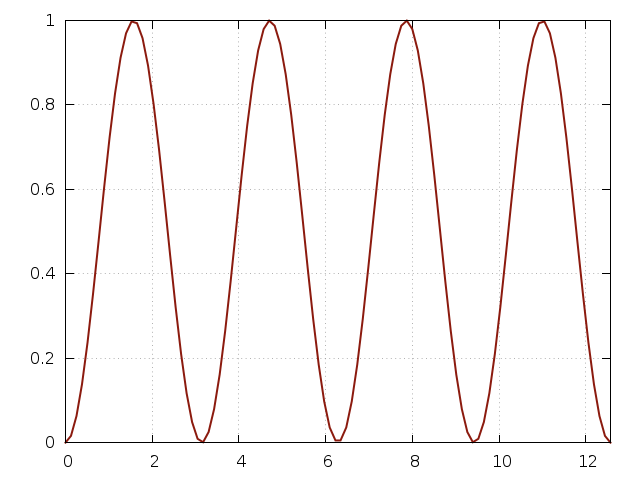
\includegraphics[scale=0.3]{1o1.png}
			\caption{$F(t) ; \omega = 1 \frac{rad}{s}$}
		\end{figure}
		
	Vamos calcular a velocidade em função do tempo $V(t)$ e a posição em função do tempo $X(t)$
	
	Sendo, pela lei de Newton $F(t) = m\frac{dv}{dt}$ vemos que:
	
	\[  V(t) - V(0)  = \int_{0}^{t} \frac{F(t') dt}{m}' \]
	
	Como $V(0)=0$:
	
	\[ V(t) = \int_{0}^{t} \frac{F_0}{m} \sin^2(\omega t')  dt' \]
	
	Usando a identidade, $\sin^2(x) = \frac{1}{2} - \frac{1}{2} \cos(2x)$ conseguimos integrar.
	
	Basta ajustar as constantes e integrar para obtemos:
		\[ V(t)= \frac{F_0}{m} \left[\frac{t}{2}-\frac{\sin(2\omega t)}{4\omega}\right] \]
		\begin{figure}[h]
			\centering
			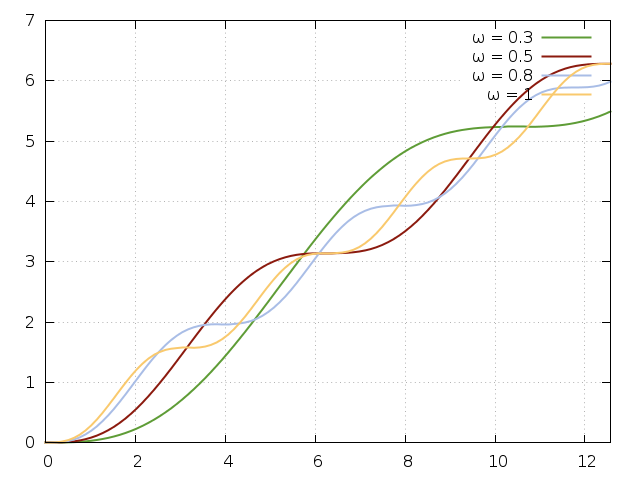
\includegraphics[scale=0.6]{1o2.png}
			\caption{$V(t)$}
		\end{figure}
		
	Agora utilizando o mesmo raciocínio para x podemos ver que:
	
	\[ X(t) - X(0) = \int_{0}^{t} V(t') dt' \]
	
	Usando $X(0)=X_0$ e substituindo $V(t)$ temos:
	
	
	\[ X(t) - X_0 = \int_{0}^{t} \left( \frac{F_0}{m} \left[\frac{t}{2}-\frac{\sin(2\omega t)}{4\omega}\right] \right)  dt' \]
	\[ X(t) - X_0 = \frac{F_0}{m} \left[ \int_{0}^{t} \frac{t}{2} dt' - \int_{0}^{t}  \frac{\sin(2\omega t)}{4\omega} dt'\right] \]
	Fazendo substituição em $2\omega t $
	\[ X(t) - X_0 = \frac{F_0}{m} \left[ \frac{t^2}{4} + \frac{\cos(2\omega t)}{8\omega^2} - \frac{1}{8\omega^2}\right] \]
	\[ X(t)= \frac{F_0}{m} \left[ \frac{t^2}{4} + \frac{\cos(2\omega t)}{8\omega^2} - \frac{1}{8\omega^2}\right] + X_0 \]
		
		
		\begin{figure}[h]
			\centering
			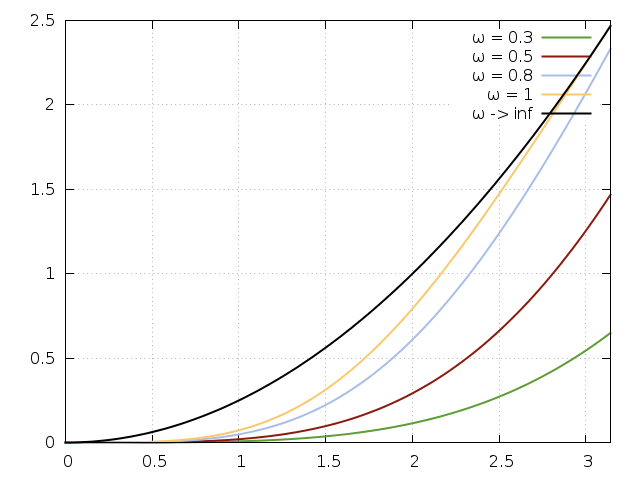
\includegraphics[scale=0.6]{1o3.png}
			\caption{$X(t)$}
		\end{figure}
		
		Note que quanto maior a frequência mais próximo de uma parábola o gráfico se aproxima, ou seja quando $\omega$ é muito grande temos um regime próximo a uma
		força constante.
		
		É fácil notar ao calcular o limite quando $\omega $ vai a infinito.
		
		\[ \lim_{\omega \rightarrow \infty} \frac{F_0}{m} \left[ \frac{t^2}{4} + \frac{\cos(2\omega t)}{8\omega^2} - \frac{1}{8\omega^2}\right] + X_0 \] = 		
		\[ \frac{F_0}{m} \frac{t^2}{4} + X_0 \]
		
		Obtemos assim a parábola.
		
		Podemos associar este problema a qualquer problema prático envolvendo uma força constante, simplismente trocando a constante por algo que vibra em torno da constante
		com o intuito de tornar a análise mais profunda e detalhada, porém funções trigonométricas ainda que representem a oscilação e a faixa de erro de uma grandeza são previsíveis
		e pouco próximas da realidade para sistemas reais que exigem esse nível de detalhe. 
		\begin{figure}[h]
			\centering
			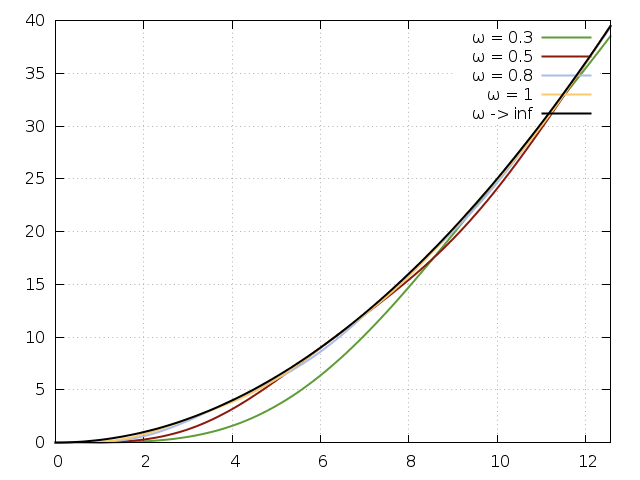
\includegraphics[scale=0.6]{1o4.png}
			\caption{$X(t)$}
		\end{figure}


	\end{document}
